\documentclass[11pt]{article}
\usepackage[T1]{fontenc}
\usepackage[utf8]{inputenc}
\usepackage{lmodern}
\usepackage[margin=1.05in]{geometry}
\usepackage{amsmath,amssymb,amsthm,mathtools}
\usepackage{microtype}
\usepackage{tikz}
\pdfinfoomitdate=1
\pdftrailerid{}
\pdfsuppressptexinfo=-1
\input{glyphtounicode}
\pdfgentounicode=1
\pdfglyphtounicode{parenleftbig}{0028}
\pdfglyphtounicode{parenrightbig}{0029}
\pdfglyphtounicode{vextenddouble}{2016}
\pdfglyphtounicode{bardbl}{2016}
\pdfglyphtounicode{slashbig}{002F}
\pdfglyphtounicode{parenleftbigg}{0028}
\pdfglyphtounicode{parenrightbigg}{0029}
\pdfglyphtounicode{parenleftBigg}{0028}
\pdfglyphtounicode{parenrightBigg}{0029}
\pdfglyphtounicode{braceleftBigg}{007B}
\pdfglyphtounicode{bracerightBigg}{007D}
\pdfglyphtounicode{angbracketleftBig}{27E8}
\pdfglyphtounicode{angbracketrightBig}{27E9}
\pdfglyphtounicode{circlemultiplydisplay}{2A02}
\pdfglyphtounicode{summationtext}{2211}
\pdfglyphtounicode{producttext}{220F}
\pdfglyphtounicode{summationdisplay}{2211}
\pdfglyphtounicode{productdisplay}{220F}
\pdfglyphtounicode{radicalbig}{221A}
\pdfglyphtounicode{radicalBig}{221A}
\pdfglyphtounicode{mapsto}{007C}
\pdfglyphtounicode{Delta}{0394}
\pdfglyphtounicode{openbullet}{2218}
\usepackage[hidelinks,pdfusetitle]{hyperref}
\usepackage{bookmark}
\newcommand{\C}{\mathbb C}
\newcommand{\N}{\mathbb N}
\newcommand{\R}{\mathbb R}
\newcommand{\Z}{\mathcal Z}
\newcommand{\sa}{\mathrm{sa}}
\newcommand{\id}{\mathrm{id}}
\newcommand{\otmax}{\otimes_{\max}}
\newcommand{\otmin}{\otimes_{\min}}
\newtheorem{theorem}{Theorem}[section]
\newtheorem{proposition}[theorem]{Proposition}
\newtheorem{lemma}[theorem]{Lemma}
\newtheorem{corollary}[theorem]{Corollary}
\theoremstyle{definition}
\newtheorem{definition}[theorem]{Definition}
\theoremstyle{remark}
\newtheorem{remark}[theorem]{Remark}
\numberwithin{equation}{section}
\DeclareMathOperator{\spanR}{span_{\R}}
\DeclareMathOperator{\rank}{rank}
\title{The Kirchberg--R\o rdam character criterion}
\author{OpenAI}
\date{September 25, 2026}
\begin{document}
\maketitle
\begin{abstract}
We prove the Kirchberg--R\o rdam character criterion: for every free
ultrafilter on $\N$, a nonzero unital separable complex $C^*$-algebra
absorbs the Jiang--Su algebra if and only if its norm central-sequence
algebra has no characters. We also prove that the infinite minimal tensor
power of every nonzero unital separable complex $C^*$-algebra without
characters is $\Z$-stable and contains a unital copy of $\Z$.
\end{abstract}
\section{Introduction}\label{sec:introduction}

For a nonzero unital $C^*$-algebra $A$ and a free ultrafilter $\omega$ on
$\N$, write
\[
 A_\omega=\ell^\infty(\N,A)\big/
 \{(a_n):\lim_{n\to\omega}\|a_n\|=0\},
 \qquad F_\omega(A)=A_\omega\cap A',
\]
where $A$ is identified with its diagonal image in $A_\omega$. A
\emph{character} is a nonzero $*$-homomorphism to $\C$; on a unital algebra
it is automatically unital. We write $\Z$ for the Jiang--Su algebra
introduced by Jiang and Su \cite{JS}. An algebra is \emph{$\Z$-stable}
if it is isomorphic to its minimal tensor product with $\Z$.

Tensorial absorption can be recognized through central copies of the
absorbed algebra. The theory of strongly self-absorbing algebras developed
by Toms and Winter makes this principle precise \cite{TW}. In the case
of $\Z$, Kirchberg and R\o rdam proved that a unital separable algebra
is $\Z$-stable exactly when its norm central-sequence algebra contains,
with the same unit, a separable subhomogeneous algebra without characters
\cite[Theorem~2.5]{KR}. Here subhomogeneity means a common finite bound
on the dimensions of irreducible representations. The absence of
characters on that subalgebra plainly forces the same absence on the
whole central-sequence algebra. The question is whether this elementary
obstruction is already sufficient.

Kirchberg and R\o rdam asked whether the absence of characters on
$F_\omega(A)$ characterizes Jiang--Su absorption among unital separable
$C^*$-algebras \cite[Question~3.1]{KR}. Their work relates this question to
tensor powers of algebras without characters
\cite[Question~3.7 and Proposition~3.9]{KR}. The character question also
appears as Problem~LXXX in the recent collection of
Schafhauser, Tikuisis, and White \cite[Section~22]{STW}. We prove the
proposed characterization.

\begin{theorem}\label{thm:main}
Let $A$ be a nonzero unital separable complex $C^*$-algebra, and let
$\omega$ be any free ultrafilter on $\N$. Then
\[
 F_\omega(A)\text{ has no characters}
 \quad\Longleftrightarrow\quad A\cong A\otmin\Z.
\]
\end{theorem}

The hypothesis uses the norm central-sequence algebra. The theorem applies
to all such $A$, with no nuclearity, simplicity, trace, dimension, or
comparison assumption. Its main ingredient is the following finite
construction, in which separability is unnecessary.

\begin{theorem}\label{thm:finite}
Let $D$ be a nonzero unital complex $C^*$-algebra without characters. There
is an integer $m\ge1$ and a unital $*$-homomorphism
\[
 I(2,3)\longrightarrow D^{\otimes_{\max}m},
\]
where
\[
I(2,3)=\{f\in C([0,1],M_2\otimes M_3):
 f(0)\in M_2\otimes1_3,\ f(1)\in1_2\otimes M_3\}.
\]
\end{theorem}

The exponent depends on $D$. The conclusion is a unital homomorphism,
not a claim that this finite tensor power itself absorbs $\Z$.
Its image is subhomogeneous and characterless, even if the homomorphism
has a kernel. These are precisely the properties needed for the
central-sequence application. They also give the following consequence.

\begin{corollary}[Infinite minimal tensor powers]\label{cor:infinite-tensor}
Let $D$ be a nonzero unital separable complex $C^*$-algebra without
characters, and write
\[
 B=D^{\otimes_{\min}\infty}
 :=\varinjlim_{n\ge1}
 \bigl(D^{\otimes_{\min}n},\,x\longmapsto x\otimes1_D\bigr).
\]
Then $B\cong B\otmin\Z$, and $B$ contains a unital copy of $\Z$.
\end{corollary}

Separability is needed for this application of Dadarlat--Toms, but neither
nuclearity nor simplicity is assumed. The absorption conclusion concerns
the infinite minimal tensor power, not a finite power.

\subsection{Earlier results and the remaining construction}

Dadarlat and Toms connected Jiang--Su absorption with infinite tensor
powers \cite{DT}. Their Theorem~1.1 shows that the infinite minimal
tensor power of a unital separable algebra is $\Z$-stable whenever
it contains a same-unit subhomogeneous characterless subalgebra. The
construction in their Theorem~6.2 gives, for each fixed prime
dimension-drop algebra, a unital map into any separable recursive
subhomogeneous algebra of finite topological dimension whose minimum
matrix size is sufficiently large relative to that dimension.
Our finite theorem begins only with absence of characters on $D$ and
uses maximal tensor products, so it must construct the required
subhomogeneous image without such a structural hypothesis.

A positive element is \emph{full} if the closed two-sided ideal it
generates is the whole ambient algebra. Several regularity criteria
explain why finding the subhomogeneous image is useful.
Robert and Tikuisis showed that two full orthogonal positive elements in
the central-sequence algebra suffice for absorption when the original
separable algebra has finite nuclear dimension \cite[Theorem~1.2]{RT}.
More recently, Perera, Thiel, and Vilalta characterized $\Z$-stability
of separable algebras by purity of the central-sequence algebra
\cite[Theorem~3.6]{PTV}.
Purity imposes comparison and divisibility conditions on its Cuntz
semigroup. The present argument assumes neither finite nuclear dimension
nor these comparison and divisibility properties.

The companion \cite[Theorem~1.4]{Fixed231} proves that a finite maximal tensor power
of every nonzero unital characterless algebra contains two full
orthogonal positive elements, without separability or nuclearity.
Its Gaussian and pure-state-excision proof is different from the
representation-label argument developed below. We also use the
companion's commuting-copy lemma \cite[Lemma~9.3]{Fixed231}, with the
primary reindexing provenance in
\cite[Proposition~2.2 and Corollary~2.3]{KR}.

The bridge from full orthogonal elements to a homomorphism from the matrix
cone $C_0((0,1])\otimes M_2$ that sends $t\mapsto t e_{11}$ to a full
element already appears in the proof of
\cite[Proposition~6.1]{KR}. We give a complete
construction using representation-stable tensor labels. A matrix-cone
map can equivalently be viewed as a completely positive contractive
order-zero map on a matrix algebra, meaning one that preserves
orthogonality of positive elements,
as in Winter and Zacharias \cite[Corollary~4.1]{WZ}; below we construct
the cone homomorphism directly. Fullness of its first matrix corner is
not by itself the dimension-drop criterion. The additional task is to
produce two \emph{exactly equivalent} orthogonal positive contractions,
of the form $v^*v$ and $vv^*$ for a single element $v$, and compare
their unit defect with a positive cutoff of one of them.
This is the input to the stable-rank-free implication of
R\o rdam and Winter \cite[Proposition~5.1, (ii)$\Rightarrow$(iv)]{RW},
whose needed form is proved explicitly in Section~\ref{sec:rw}.

\subsection{Proof overview}

We give the finite construction in two stages. First, a finite-dimensional
space of selfadjoints detects noncommutativity in every representation of
$D$. An incidence argument supplies tensor labels that remain linearly
independent after arbitrary rank-at-least-two maps on the individual legs.
These labels yield two selfadjoints that do not commute in any irreducible
representation of a suitable tensor power. A double commutator then has
full positive and negative parts, and a second use of the labels assembles
finitely many bridges between them into one full square-zero element.

Second, the square-zero element gives a matrix-cone homomorphism with a full
first corner. A
continuous simplex of embeddings of $M_2$ organizes this cone across a
finite tensor power. Two orthogonal equivalent positive elements leave a
defect concentrated near the origin of a cube. Disjoint regions near its
coordinate axes support elements that absorb this defect after a further
finite amplification. The resulting comparison is precisely the one
required by the R\o rdam--Winter dimension-drop criterion. This comparison
is the step that turns full orthogonal elements into a unital $I(2,3)$ map.

Section~\ref{sec:preliminaries} records the comparison conventions and
structural criteria, with the dimension-drop conversion proved in
Section~\ref{sec:rw}. Section~\ref{sec:tensor} constructs this cone homomorphism,
and Section~\ref{sec:dimension-drop} proves the finite comparison.
Section~\ref{sec:application} deduces both theorems and
Corollary~\ref{cor:infinite-tensor}. All tensor exponents and comparison
constants are allowed to depend on the algebra $D$.

\section{Preliminaries}\label{sec:preliminaries}

\subsection{Tensor products and positive elements}
All algebras are complex. All tensor products in the construction are
\emph{maximal}, and we abbreviate $D^{\otimes_{\max}n}$ to $D^{\otimes n}$.
We specify minimal tensor products explicitly. Algebraic tensor products
are denoted by $\odot$ over $\C$ and by $\otimes_{\R}$ over $\R$.
Representations called irreducible are nonzero and nondegenerate, hence
unital when the represented algebra is unital. An element is \emph{full}
if its generated closed two-sided ideal is the whole algebra. Equivalently,
it is nonzero in every irreducible representation: a proper ideal has a
nonzero irreducible representation of its quotient.

For positive elements in finite matrix algebras over a unital algebra $B$,
write $a\precsim b$ if, after adjoining zero corners as necessary, there
are matrices $x_j$ with $x_j^*b x_j\to a$ in norm. Write $[a]$ for the
resulting Cuntz equivalence class. Thus $[a]\le[b]$ means
$a\precsim b$, and addition is induced by direct sum. We use only the
following elementary rules:
\begin{enumerate}
\item $[v^*v]=[vv^*]$ for every rectangular matrix $v$;
\item if $a_1,\ldots,a_l$ are positive and pairwise orthogonal, then
$[\sum_i a_i]=\sum_i[a_i]$;
\item comparison and addition are preserved by $*$-homomorphisms and by
external tensoring with a fixed positive element, including for maximal
tensor products.
\end{enumerate}
For the first rule, with $b=v^*v$, the matrices
$x_\gamma=v(b+\gamma)^{-1/2}$ satisfy
$x_\gamma^*(vv^*)x_\gamma=b^2(b+\gamma)^{-1}\to b$ as
$\gamma\downarrow0$; apply the same argument to $v^*$ for the converse.
For the second rule, apply the first to the row
$(a_1^{1/2},\ldots,a_l^{1/2})$. For the third rule, apply a homomorphism to
the witnesses, or tensor them with the unit of the other algebra. The norm
estimate for the resulting error is at most the original error times the
norm of the fixed positive tensor factor. Direct sums agree under the
canonical matrix identifications. These rules use no cancellation or
regularity of the Cuntz order. We also use $[a]\le[1_B]$ for $a\in B_+$,
which follows from the exact witness $a^{1/2}$.

\subsection{The dimension-drop criterion}
We say that positive elements $a_1,a_2\in B$ are \emph{equivalent} if
$a_1=v^*v$ and $a_2=vv^*$ for one $v\in B$. This is the exact relation
required in the next proposition.

\begin{proposition}[R\o rdam--Winter]\label{prop:rw}
Let $B$ be a unital $C^*$-algebra. Suppose that $a_1,a_2\in B$ are
orthogonal positive contractions with $a_1=v^*v$, $a_2=vv^*$ for some
$v\in B$, and that, for some $\varepsilon>0$,
\[
 1_B-a_1-a_2\precsim(a_1-\varepsilon)_+.
\]
Then there is a unital $*$-homomorphism $I(2,3)\to B$.
\end{proposition}

This is \cite[Proposition~5.1, (ii)$\Rightarrow$(iv), with $n=2$]{RW}.
Section~\ref{sec:rw} supplies a complete proof using their method, with
the support projections, scalar endpoint fiber, and weighted flip
identity made explicit.
The stable-rank-one hypothesis appearing elsewhere in that proposition is
needed only for (i)$\Rightarrow$(ii). It is not a hypothesis of the
implication stated here. Orthogonality ensures $a_1+a_2\le1_B$, so the
defect in the display is positive.

\subsection{Central-sequence inputs}
We use the following results of Kirchberg and R\o rdam for the fixed free
ultrafilter $\omega$.

\begin{proposition}[Kirchberg--R\o rdam]\label{prop:kr}
Let $A$ be a nonzero unital separable $C^*$-algebra.
\begin{enumerate}
\item If $D\subset F_\omega(A)$ is separable and contains the ambient
unit, then for every $m\ge1$ there is a unital $*$-homomorphism
$D^{\otimes_{\max}m}\to F_\omega(A)$.
\item $A\cong A\otmin\Z$ if and only if $F_\omega(A)$ contains, with
the ambient unit, a separable subhomogeneous $C^*$-algebra without
characters.
\end{enumerate}
\end{proposition}

The first assertion is the unital specialization of the commuting-copies
lemma in \cite[Lemma~9.3]{Fixed231}, whose primary source is
\cite[Proposition~2.2 and Corollary~2.3]{KR}. For unital $A$, the
annihilator ideal used in that companion is zero: an element annihilating
every element of $A$ annihilates its unit. Thus its $F(A)$ is precisely
the norm central-sequence algebra used here. This particular lemma has
no nuclear-dimension assumption. We include the short specialization
to make its quantifiers explicit.

\begin{proof}[Proof of Proposition~\ref{prop:kr}(1)]
For any separable subalgebra $E\subset F_\omega(A)$, we construct a
unital map from $D$ into $F_\omega(A)\cap E'$. Choose a countable dense
unital $*$-subalgebra $D_0\subset D$ over $\mathbb Q+i\mathbb Q$.
For every $x\in D_0$, choose a bounded lift $(a_l^x)_l$ in $A$ with
$\sup_l\|a_l^x\|\le2\|x\|$, using the zero lift for $x=0$ and the
constant unit lift for $x=1$. Such choices follow from the quotient norm,
by truncating coordinate norms without changing the ultrapower class.
All additive, rational-complex scalar, multiplicative and adjoint
relation defects tend to zero in norm along $\omega$.

Choose a countable dense subset of $A$ and bounded lifts $(b_s^j)_s$
of a countable dense subset of $E$. Enumerate the relation-defect tests
and the tests for centrality of the $a_l^x$ against the chosen subset
of $A$. For each output index $s$, choose $l(s)$ so that the first $s$
tests hold within $1/s$, and so that
\[
 \|[a_{l(s)}^x,b_s^j]\|<1/s
\]
for the first $s$ pairs $(x,j)$ in an enumeration. Each of the finitely
many requirements holds on an $\omega$-large set of old indices $l$:
for this fixed $s$, each $b_s^j$ is a fixed element of $A$, so original
centrality applies. Their finite intersection is nonempty.

The new sequences $(a_{l(s)}^x)_s$ are central and satisfy every
algebraic relation in the ordinary limit, hence along the arbitrary
free ultrafilter $\omega$. Their classes define a unital
rational-complex $*$-homomorphism on $D_0$ into $F_\omega(A)\cap E'$.
The uniform bound $2\|x\|$ extends it continuously to a complex unital
$*$-homomorphism on $D$. Starting with the given copy of $D$ and taking
$E$ successively to be the algebra generated by the earlier images
produces any prescribed finite number of commuting unital images.
The universal property of the maximal tensor product gives (1).
Injectivity of the reindexed maps is not needed.
\end{proof}

The second assertion is \cite[Theorem~2.5]{KR}. Here
\emph{subhomogeneous} means that the dimensions of all irreducible
representations have a common finite bound. In particular, this input
does not replace norm central sequences by a tracial ultrapower or
impose nuclearity on $A$.

\section{The dimension-drop criterion without stable rank one}
\label{sec:rw}

This section proves the implication of R\o rdam and Winter
\cite[Proposition~5.1, (ii)$\Rightarrow$(iv)]{RW} used in the finite
construction. We retain their order-zero and flip-path method, while
making the support projections and endpoint domains explicit. The
argument applies to an arbitrary unital $C^*$-algebra.

For $b\ge0$, write $\operatorname{Her}(b)=\overline{bBb}$.
Support projections and polar decompositions will be taken in $B^{**}$.
They need not belong to $B$; we will verify membership in $B$ whenever
they are used to construct an element of the original algebra.

\begin{lemma}\label{lem:rw-exact-cut}
If $a,b\in B_+$ satisfy $a\precsim b$, then for every $\delta>0$
there is $z\in B$ such that
\[
 z^*z=(a-\delta)_+,
 \qquad zz^*\in\operatorname{Her}(b).
\]
\end{lemma}
\begin{proof}
Since $a,b$ lie in $B$, compression of stabilized comparison
witnesses to their $(1,1)$ entries gives witnesses in $B$ itself.
Choose $x\in B$ with $\|a-x^*bx\|<\eta<\delta$, and put
$e=(a-\delta)_+$ and $y=b^{1/2}xe^{1/2}$. Then
\[
 T=y^*y\ge e^{1/2}(a-\eta)e^{1/2}
       \ge(\delta-\eta)e,
 \qquad T\le\|x^*bx\|e.
\]
Thus $T$ and $e$ have the same support. If $y=uT^{1/2}$ is the polar
decomposition, set $z=ue^{1/2}$ in $B^{**}$. To see that $z\in B$,
approximate it by
\[
 z_\tau=y(T+\tau)^{-1/2}e^{1/2}\in b^{1/2}B,
 \qquad \tau>0.
\]
Writing $f_\tau(t)=1-\sqrt{t/(t+\tau)}$, the domination of $e$ by
$T$ gives
\[
 \|z-z_\tau\|^2
 \le\|f_\tau(T)e f_\tau(T)\|
 \le\frac{\sup_{t\ge0}t f_\tau(t)^2}{\delta-\eta}
 \le\frac{\tau}{\delta-\eta}.
\]
No commutation of $e$ with $T$ is used here. Hence $z\in B$,
$z^*z=e$, and $zz^*$ is a norm limit of elements of
$b^{1/2}Bb^{1/2}$, as required.
\end{proof}

We shall use a concrete description of order-zero maps. If
$x_1,\ldots,x_q$ are contractions with
$x_i x_j^*=\delta_{ij}h$ for a positive contraction $h$, then
\[
 \alpha(e_{ij})=x_i^*x_j
\]
defines a completely positive contractive order-zero map from $M_q$.
Indeed, complete positivity follows from this Gram formula. The
positive elements $x_i^*x_i$ are orthogonal, so their sum $H$ is a
contraction; multiplication gives
$\alpha(e_{ij})\alpha(e_{kl})=\delta_{jk}H\alpha(e_{il})$.
This identity proves preservation of orthogonality. It also gives a
supporting homomorphism $\bar\alpha:M_q\to B^{**}$ with
\[
 \alpha(x)=H\bar\alpha(x)=\bar\alpha(x)H,
 \qquad \bar\alpha(1_q)=\operatorname{supp}(H).
\]
For completeness, its matrix units are the strong limits of
$\alpha(e_{ij})(H+\tau)^{-1}$ as $\tau\downarrow0$. The displayed
multiplication identity and
$\alpha(e_{ij})^*\alpha(e_{ij})\le H^2$ verify their boundedness,
matrix-unit relations, and stated support.

\begin{lemma}\label{lem:rw-commuting-maps}
Let $\alpha:M_3\to B$ and $\beta:M_2\to B$ be completely positive
contractive maps with commuting ranges, satisfying
$\psi(x)\psi(y)=\psi(1)\psi(xy)$ for $\psi=\alpha,\beta$.
If
$\alpha(1_3)+\beta(1_2)=1_B$, there is a unital homomorphism
$I(2,3)\to B$.
\end{lemma}
\begin{proof}
This is the order-zero presentation used in
\cite[Proposition~2.5]{RW}; we include the verification.
The canonical maps into $I(2,3)$ are
\[
 \alpha_0(y)(t)=t(1_2\otimes y),\qquad
 \beta_0(x)(t)=(1-t)(x\otimes1_3).
\]
Their generated algebra contains the scalar function $t$, and products
of their entries generate the ideal $C_0((0,1),M_2\otimes M_3)$.
Their endpoint values also generate $M_2\oplus M_3$. Consequently
they generate all of $I(2,3)$.

Put $E=C^*(\alpha(M_3),\beta(M_2),1_B)$. The element
$\alpha(1_3)$ is central in $E$. In any irreducible representation
of $E$ it is a scalar $r\in[0,1]$. If $0<r<1$, the rescaled maps
$r^{-1}\alpha$ and $(1-r)^{-1}\beta$ in this representation are
commuting unital matrix homomorphisms, and hence define a representation
of $M_2\otimes M_3$. At $r=0$ only the $M_2$ map remains, and at
$r=1$ only the $M_3$ map remains. These assertions follow either from
the supporting homomorphisms or directly from the order-zero
multiplication identity.

It follows that substitution of $\alpha,\beta$ for
$\alpha_0,\beta_0$ in a noncommutative $*$-polynomial is bounded in
norm by the norm of the polynomial in $I(2,3)$: test in each
irreducible representation of $E$ and use the corresponding evaluation
at $r$. Substitution is therefore well defined and extends from the
dense generated algebra to the required unital homomorphism.
\end{proof}

\begin{proof}[Proof of Proposition~\ref{prop:rw}]
\emph{Exact relations from the comparison.}
Write $a_1=w^*w$ and $a_2=ww^*$ for the equivalence witness.
Decreasing $\varepsilon$ if necessary, assume $0<\varepsilon<1$.
Let $f(t)=\min\{t/\varepsilon,1\}$ and put
$s_1=f(a_1)^{1/2}$. If $w^*=u_0a_2^{1/2}$ is its polar
decomposition, put $s_2=u_0f(a_2)^{1/2}$. This belongs to $B$:
it equals $w^*q(a_2)$, where the continuous function
$q(t)=\sqrt{f(t)/t}$ for $t>0$ is assigned the value
$\varepsilon^{-1/2}$ at zero. Thus
\[
 s_i s_j^*=\delta_{ij}s_1^2,\qquad
 d:=s_1^*s_1+s_2^*s_2=f(a_1)+f(a_2).
\]
Here the off-diagonal products vanish because the initial positive
elements are orthogonal. Writing $c=1-a_1-a_2$, functional calculus
in the commuting algebra generated by $a_1,a_2$ gives
\[
 a:=1-d=\varepsilon^{-1}(c-(1-\varepsilon))_+.
\]
Apply Lemma~\ref{lem:rw-exact-cut} to $c\precsim(a_1-\varepsilon)_+$,
with $\delta=1-\varepsilon$, and divide its element by
$\sqrt\varepsilon$. We obtain a contraction $v\in B$ satisfying
\begin{equation}\label{eq:rw-relations}
 v^*v=a=1-d,\qquad vv^*\in\operatorname{Her}((a_1-\varepsilon)_+),
 \qquad s_1^2vv^*=vv^*.
\end{equation}
In particular $s_1v=v$, $s_2v=0$, and $av=0$.
The initial and final support relations also give
$ds_i=s_1^2s_i=s_id$; hence $a$ commutes with the $s_i$.
The Gram construction gives $\rho:M_2\to B$ with
$\rho(e_{ij})=s_i^*s_j$ and $\rho(1_2)=d$.
Write $\sigma$ for its supporting homomorphism and
$p=\operatorname{supp}(d)$.

\emph{Two orthogonal copies of the defect algebra.}
Let $v=ua^{1/2}$ be the polar decomposition and
$e=u^*u=\operatorname{supp}(a)$. Set
\[
 r_i=s_i^*u=\sigma(e_{i1})u\quad(i=1,2),
 \qquad R=r_1r_1^*+r_2r_2^*.
\]
The second formula for $r_i$ follows from $du=u$ and $s_1u=u$.
Direct multiplication gives
\begin{equation}\label{eq:rw-corners}
 r_i^*r_j=\delta_{ij}e,\qquad
 dr_i=r_i,\qquad R\le p,\qquad R\perp e,\qquad
 \sigma(e_{jk})r_i=\delta_{ki}r_j.
\end{equation}
For $R\perp e$, note that $a$ commutes with each $s_i$ (because
$d$ does) and $au=0$. The map
\[
 \varphi:\operatorname{Her}(a)\longrightarrow B,
 \qquad \varphi(b)=\sum_{i=1}^2 r_i b r_i^*
\]
is a homomorphism by \eqref{eq:rw-corners}. Its values belong to
$B$: approximate $b\in\operatorname{Her}(a)$ by
$a^{1/2}b_m a^{1/2}$ and use $ua^{1/2}=v$ to see that
$ubu^*\in B$. The same approximation, with one outer factor omitted,
shows that $ub\in B$.
The same relations show
\begin{equation}\label{eq:rw-phi}
 \varphi(b)r_i=r_i b,\qquad
 [\varphi(b),\sigma(M_2)]=0,\qquad
 \varphi(\operatorname{Her}(a))\perp\operatorname{Her}(a).
\end{equation}

Here $\varphi(b)=\sum_i r_i b r_i^*$ places the same defect element in
the two ranges of the $r_i$, while $\sigma(e_{jk})$ acts on their index
$i$. To obtain the other coordinate, we use sections on $[0,1]$ with values
in $M_2$, evaluated at $d$, that are scalar at zero and vanish at one.
The scalar value accounts for the corner outside $p=\operatorname{supp}(d)$;
vanishing at one keeps the evaluated section in $\operatorname{Her}(1-d)$.
Define
\[
 D_1=\{F\in C([0,1],M_2):F(0)\in\mathbb C1_2,\ F(1)=0\},
\]
and let $c_F$ be the scalar with $F(0)=c_F1_2$. Since $d$ commutes
with $\sigma(M_2)$, continuous functional calculus defines
$\bar\lambda(F)=\sum_{i,j}F_{ij}(d)\sigma(e_{ij})$ in $pB^{**}p$.
The required homomorphism is
\begin{equation}\label{eq:rw-lambda}
 \lambda(F)=\bar\lambda(F)+c_F(1-p).
\end{equation}
The extra summand retains the scalar fiber at zero. In particular
$\lambda(f1_2)=f(d)$ for scalar $f$ vanishing at one.
The algebra $D_1$ is generated by $(1-t)1_2$ and
$t(1-t)x$, $x\in M_2$. Their images are respectively $a$ and
$a\rho(x)$, so $\lambda$ takes values in $\operatorname{Her}(a)$.
This also verifies membership in $B$, without assuming $p\in B$.

Let
\[
 D_2=\{F\in C([0,1],M_2\otimes M_2):
                   F(0)\in\mathbb C1_4,\ F(1)=0\}.
\]
It is a subalgebra of $D_1\otimes M_2$. By
\eqref{eq:rw-phi}, the commuting product of
$\varphi\circ\lambda$ and $\sigma$ defines a homomorphism on
$D_1\otimes M_2$; denote its restriction to $D_2$ by $\gamma$.
Its range lies in $B$: since $d\varphi(b)=\varphi(b)$,
$\varphi(b)\sigma(x)=\varphi(b)\rho(x)\in B$.
Its support projection is $R$, because its range is supported there
and contains $\varphi(a)$, which has support $R$.

The product defining $\gamma$ pairs this transported section action with
the action of $\sigma$ on the copy index. A weighted flip will interchange
them only on the overlap needed for the final commutation calculation.

\emph{The flip where the two pieces overlap.}
Let $F\in M_2\otimes M_2$ be the flip unitary. Choose a continuous
function $\theta:[0,1]\to[0,1]$ that is zero on $[0,1/3]$ and one
on $[2/3,1]$, and set
\[
 U(t)=\frac{1+F}{2}+e^{i\pi\theta(t)}\frac{1-F}{2}.
\]
This is an ordinary unitary path, equal to $1$ near zero and to
$F$ on $[2/3,1]$. It is a multiplier of $D_2$. The multiplier
extension of $\gamma$ sends it to a unitary $w_0$ in the corner
$RB^{**}R$; put $W=w_0+1-R$.

Let $g(t)=1$ for $0\le t\le2/3$ and $g(t)=3(1-t)$ otherwise.
Put
\[
 h=\lambda(g1_2)=g(d),\qquad k=\varphi(h),\qquad l=1-h-k.
\]
The elements $h,k$ are orthogonal positive contractions, and
$g(t)\ge1-t$ implies $0\le l\le d$. Also $kW=Wk$ and
\[
 k^\alpha W=\gamma(g^\alpha U)\in B\qquad(\alpha>0).
\]
The formula is legitimate because $g^\alpha U\in D_2$.
Define
\[
 x_i=h^{1/2}r_i^*W\quad(i=1,2),\qquad x_3=h^{1/2}.
\]
These elements belong to $B$: for $i\le2$ use the factorization
\[
 x_i=(r_i^*k^{1/4})(k^{1/4}W),\qquad
 r_i^*k^{1/4}=h^{1/4}r_i^*\in B.
\]
By \eqref{eq:rw-corners}, $R\perp e$, and unitarity of $W$,
\[
 x_i x_j^*=\delta_{ij}h\quad(1\le i,j\le3),\qquad
 \sum_{i=1}^3x_i^*x_i=h+k.
\]
Thus $\alpha(e_{ij})=x_i^*x_j$ defines an order-zero map
$\alpha:M_3\to B$ with $\alpha(1_3)=h+k$.

Since $h,k$ commute with $\sigma(M_2)$ and $0\le l\le d$, the
formula $\beta(y)=l\sigma(y)$ defines an order-zero map
$\beta:M_2\to B$. To justify its range directly, $l$ vanishes on
the spectral subspace of $d$ for $[0,2/3]$, since $h=1$ there and
$hk=0$. Choose a continuous scalar function $j$ that equals $1/t$
for $t\ge2/3$. Then
$\beta(y)=lj(d)\rho(y)\in B$.
Since $lp=l$, we have
$\alpha(1_3)+\beta(1_2)=1$.

It remains to check that their ranges commute. This is precisely
where the flip is needed. The scalar function $Q=g(1-g)$ vanishes
at both endpoints and is supported where $U=F$. Therefore
\[
 Q(t)(1\otimes y)U(t)^*
   =U(t)^*Q(t)(y\otimes1),\qquad y\in M_2.
\]
Both sides are elements of $D_2$. Applying $\gamma$ gives the
well-defined identity
\begin{equation}\label{eq:rw-weighted-flip}
 k(1-k)\sigma(y)W^*
       =W^*\varphi\bigl(\lambda(Q\otimes y)\bigr).
\end{equation}
In particular, no constant nonscalar section is evaluated by
$\lambda$. For $i=1,2$, put
$C_i=\alpha(e_{i3})=W^*r_i h$. Using
\eqref{eq:rw-phi} and \eqref{eq:rw-weighted-flip}, we obtain
\[
\begin{aligned}
 \beta(y)C_i
 &=k(1-k)\sigma(y)W^*r_i\\
 &=W^*r_i\lambda(Q\otimes y)\\
 &=W^*r_i h(1-h)\sigma(y)
  =C_i\beta(y).
\end{aligned}
\]
Here $\lambda(Q\otimes y)=Q(d)\sigma(y)$ because $Q(0)=0$;
the last equality uses $hk=0$.

The $C^*$-algebra generated by the $C_i$ contains $\alpha(M_3)$. Indeed,
$C_i^*C_i=h^2$ and $C_iC_i^*=\alpha(e_{ii})^2$, so their generated
algebra contains $h$, all diagonal entries, and
$A_0:=\alpha(1_3)$. Moreover
$C_iC_j^*=A_0\alpha(e_{ij})$, and multiplication by
$(A_0+\tau)^{-1}$ followed by $\tau\downarrow0$ recovers every
remaining matrix entry. The convergence follows from
$\alpha(e_{ij})=A_0\bar\alpha(e_{ij})$ and
$\|\tau A_0(A_0+\tau)^{-1}\|\le\tau$.
Thus $\alpha(M_3)$ commutes with $\beta(M_2)$.
Lemma~\ref{lem:rw-commuting-maps} completes the proof.

The construction also covers $v=0$: then $a=h=k=0$, $R=0$,
$W=1$, and $\beta$ is a unital $M_2$ homomorphism. No step requires
stable rank one or a nonzero defect.
\end{proof}

\section{A matrix-cone homomorphism with a full corner}
\label{sec:tensor}

We first construct a full square-zero element in a finite tensor power of
a unital \(C^*\)-algebra without characters. Its polar decomposition will
then give the matrix-cone homomorphism needed in the next section.
The absence of characters is detected by finitely many commutators.
The main issue is to combine those finitely many tests into one element
that survives every irreducible representation of a maximal tensor
product, including representations that are not spatial tensor products.

\subsection{Algebraic independence of commuting factors}

\begin{lemma}
\label{lem:tensor-independence}
Let \(M\subseteq B(H)\) be a von Neumann factor with \(1_M=1_H\), and let
\(B\subseteq M'\) be a unital algebra. The multiplication map
\[
 M\odot B\longrightarrow B(H),\qquad a\otimes b\longmapsto ab,
\]
is injective. Consequently, multiplication is injective on the complex
algebraic tensor product of any finite family of commuting von Neumann
factors on the same Hilbert space, all with unit \(1_H\).
\end{lemma}

\begin{proof}
Fix complex linearly independent elements \(b_1,\ldots,b_l\in B\).
It suffices to show that
\[
 S=\left\{(a_1,\ldots,a_l)\in M^{1\times l}:
                  \sum_{i=1}^l a_i b_i=0\right\}
\]
is zero. This row space is weak-operator closed and invariant under
diagonal multiplication by \(M\) on either side. The right invariance
uses \(B\subseteq M'\). Let \(J\subseteq M_l(M)\) consist of the matrices
whose rows belong to \(S\). It is a weak-operator closed left ideal:
each row of a left matrix product is an \(M\)-linear combination of the
original rows.

We give the support-projection argument for the form of this ideal.
For \(x\in J\), we have \(x^*x\in J\). Functional calculus with functions
vanishing at zero, followed by weak-operator closure, puts the support
projection of \(x^*x\) in \(J\): one may first take
\(x^*x(x^*x+\varepsilon1)^{-1}\) and then let
\(\varepsilon\downarrow0\). Finite joins of these projections also
belong to \(J\), since the join of finitely many projections is the
support of their sum. Their increasing join \(p\) therefore belongs to
\(J\); this is a net of finite joins, so no separability assumption is
involved. Every \(x\in J\) satisfies \(x=xp\), and \(p\in J\) gives
\[
                         J=M_l(M)p.
\]

For any unitary \(u\in M\), put \(U=\operatorname{diag}(u,\ldots,u)\).
Right invariance and its counterpart for \(u^*\) give \(JU=J\).
The right support projection of \(xU\) is the conjugate by \(U\) of the
right support projection of \(x\). Taking their joins gives
\[
                             U^*pU=p.
\]
Thus every entry of \(p\) belongs to the center of \(M\), and is scalar.
Each row of \(p\) is consequently a scalar relation among the independent
\(b_i\), so \(p=0\). Hence \(J=0\) and \(S=0\), proving the first assertion.

For finitely many commuting factors, apply the first assertion to one
factor and the algebra generated by the remaining factors, and induct
on their number.
\end{proof}

\begin{lemma}
\label{lem:tensor-grouped-factors}
Let \(\pi:B_1\otmax\cdots\otmax B_q\to B(H)\) be an irreducible
representation, where the \(B_j\) are nonzero unital
\(C^*\)-algebras. The weak-operator closures of the represented tensor
legs are commuting von Neumann factors. The same is true after grouping
the legs according to any partition into nonempty blocks.
\end{lemma}

\begin{proof}
Every represented block contains \(\pi(1)=1_H\). The represented blocks
commute, and this commutation persists under
weak-operator closure. A central element of the closure of one block
commutes both with that block and with every complementary block.
It therefore belongs to the commutant of the full irreducible image,
which consists of the scalars. This proves factorhood for each block.
\end{proof}

These lemmas concern algebraic tensor independence. They require neither
faithfulness of the restrictions to the tensor legs nor a spatial
decomposition of the represented factors.

\subsection{Labels that remain independent in representations}

\begin{lemma}
\label{lem:tensor-detecting-space}
Let \(D\) be a nonzero unital \(C^*\)-algebra without characters.
There is a finite-dimensional real subspace \(V\subseteq D_{\sa}\)
such that the image of \(V\) contains a noncommuting pair in every
nonzero unital representation of \(D\).
\end{lemma}

\begin{proof}
The closed ideal generated by the commutators of selfadjoint elements
is all of \(D\). Otherwise the quotient by this ideal would be a nonzero
unital commutative \(C^*\)-algebra, and a character of the quotient would
give a character of \(D\).

Choose a finite algebraic expression in these commutators within distance
less than one of \(1_D\). This expression is invertible, so the finitely
many commutators it uses already generate the unit ideal. Let \(V\) be
the real span of their selfadjoint entries. If a unital representation
sent \(V\) to a commuting space, it would annihilate all these
commutators, and hence their unit ideal. This is impossible.
\end{proof}

\begin{lemma}
\label{lem:tensor-real-labels}
Let \(V\) be a finite-dimensional real vector space with
\(m=\dim_{\R}V\ge2\). For every integer \(r\ge1\), there are \(n\ge1\)
and tensors \(x_1,\ldots,x_r\in V^{\otimes_{\R}n}\) with the following
property: whenever \(P_j:V\to E_j\) are real linear maps of rank at least
two, the tensors
\[
               (P_1\otimes\cdots\otimes P_n)(x_i),
               \qquad 1\le i\le r,
\]
are linearly independent over \(\R\).
\end{lemma}

\begin{proof}
It suffices to consider surjections \(P_j:V\to\R^2\).
Indeed, a map of rank at least two can be postcomposed, on its
finite-dimensional image, with a surjection onto \(\R^2\); a dependence
before this postcomposition would remain a dependence afterward.

Choose \(n\) such that
\[
                         2^n>2mn+r-1,
\]
and put \(W=V^{\otimes_{\R}n}\). Let
\(\mathcal P=\operatorname{Surj}(V,\R^2)^n\), an open subset of a real
vector space of dimension \(2mn\). Consider the smooth map
\[
 \begin{split}
 \Phi:\mathcal P\times S^{r-1}\times W^r
     &\longrightarrow (\R^2)^{\otimes_{\R}n},\\
 (P,u,x)&\longmapsto
 (P_1\otimes\cdots\otimes P_n)\left(\sum_{i=1}^r u_i x_i\right).
 \end{split}
\]
Its differential in the \(x\) variables is surjective everywhere:
some \(u_i\ne0\), and the tensor product of the \(P_j\) is surjective.
Thus \(\Phi^{-1}(0)\) is a smooth manifold of dimension
\[
                 2mn+r-1+rm^n-2^n<rm^n=\dim_{\R}W^r.
\]
By Sard's theorem, its projection to \(W^r\) has Lebesgue measure zero.
The manifolds here are second countable, so this assertion can be
applied on a countable atlas; no compactness of \(\mathcal P\) is needed.
Choose \(x\in W^r\) outside that projection. For this one tuple, no
nonzero real dependence occurs for any tuple of surjections: any
nonzero coefficient vector can be normalized to lie in \(S^{r-1}\).
\end{proof}

\begin{corollary}
\label{cor:tensor-represented-labels}
Let \(D\) and \(V\) be as in Lemma~\ref{lem:tensor-detecting-space}.
For each \(r\ge1\), there are \(n\ge1\) and selfadjoint elements
\(x_1,\ldots,x_r\in D^{\otimes n}\) whose images are complex linearly
independent under every irreducible representation of
\(D^{\otimes n}\otmax B\), for every nonzero unital \(C^*\)-algebra \(B\).
Here the elements \(x_i\) occupy the first \(n\) tensor legs.
\end{corollary}

\begin{proof}
Take the real tensors supplied by Lemma~\ref{lem:tensor-real-labels}
and map them naturally into \(D^{\otimes n}\). They are selfadjoint,
since they are real linear combinations of elementary tensors with
selfadjoint entries.

Fix such an irreducible representation and write \(\pi_j\) for its
restriction to the \(j\)-th copy of \(D\). Each \(\pi_j\) is unital, so
Lemma~\ref{lem:tensor-detecting-space} implies
\(\dim_{\R}\pi_j(V)\ge2\). Apply
Lemma~\ref{lem:tensor-real-labels} to the real maps
\(V\to\pi_j(V)\).

The resulting independence also holds after complexification.
Indeed, a real basis of a space of selfadjoint operators is complex
linearly independent: taking adjoints of a complex relation separates
its real and imaginary parts. Hence the complexification of each
\(\pi_j(V)\) embeds in the represented algebra. Tensoring these
injections shows that the real independent tensors remain complex
independent in the complex algebraic tensor product of the represented
legs: the latter tensor product contains the complexification of the
real tensor product injectively. By
Lemma~\ref{lem:tensor-grouped-factors} their weak closures are
commuting factors, and Lemma~\ref{lem:tensor-independence} preserves this
independence under multiplication.
\end{proof}

\subsection{A full square-zero element}

The existence of two full orthogonal positive elements in a finite
maximal tensor power is already established in
\cite[Theorem~1.4]{Fixed231}. The bridge construction below is related to
Kirchberg--R\o rdam's proof of \cite[Proposition~6.1, (i)$\Rightarrow$(v)]{KR},
which combines finitely many bridges with orthogonal full tensor labels.
Here we use representation-stable linear independence and give the full
construction of the square-zero element needed for the cone map.

The labels allow linear independence to replace orthogonality when
combining finitely many algebraic witnesses. We first construct two full
orthogonal positive elements, and then use a second label family to
retain all bridges between them in a single square-zero element.

\begin{lemma}
\label{lem:tensor-full-square-zero}
If \(D\) is a nonzero unital \(C^*\)-algebra without characters, then
some finite maximal tensor power \(P\) of \(D\) contains a full element
\(w\) satisfying \(w^2=0\) and \(\|w\|=1\).
\end{lemma}

\begin{proof}
Choose \(V\) as in Lemma~\ref{lem:tensor-detecting-space}, and let
\(v_1,\ldots,v_m\) be a real basis of \(V\). Take the labels
\(x_1,\ldots,x_m\in D^{\otimes n}\) from
Corollary~\ref{cor:tensor-represented-labels}. In
\[
                   P_0=D\otmax D^{\otimes n}\otmax D^{\otimes n}
\]
define selfadjoint elements
\[
 s=\sum_{i=1}^m v_i\otimes x_i\otimes1,
 \qquad
 t=\sum_{i=1}^m v_i\otimes1\otimes x_i.
\]
We first show that their images do not commute in any irreducible
representation \(\pi\) of \(P_0\). Denote the restrictions to the three
displayed blocks by \(\pi_0,\pi_L,\pi_R\). Their weak closures are
commuting factors by Lemma~\ref{lem:tensor-grouped-factors}, and each
of the two label families has independent images by
Corollary~\ref{cor:tensor-represented-labels}. The expansion
\[
 \pi([s,t])=
 \sum_{i,j=1}^m
       \pi_0([v_i,v_j])\,\pi_L(x_i)\,\pi_R(x_j)
\]
and Lemma~\ref{lem:tensor-independence} show that
\(\pi([s,t])=0\) would imply
\(\pi_0([v_i,v_j])=0\) for all \(i,j\).
This contradicts the defining property of \(V\) for the unital
representation \(\pi_0\). Independence of the images of the \(v_i\)
themselves is not required.

Set \(z=[s,[s,t]]\), which is selfadjoint. We claim that both \(z_+\)
and \(z_-\) are full in \(P_0\). Fix an irreducible representation
\(\pi\), and suppose first that \(\pi(z)\ge0\). For every vector
\(\xi\), the real function
\[
 f_\xi(\lambda)=
 \left\langle e^{i\lambda\pi(s)}\pi(t)e^{-i\lambda\pi(s)}
                       \xi,\xi\right\rangle,\qquad \lambda\in\R,
\]
is bounded and twice continuously differentiable, with
\[
 f_\xi''(\lambda)=
 -\left\langle e^{i\lambda\pi(s)}\pi(z)e^{-i\lambda\pi(s)}
                       \xi,\xi\right\rangle\le0.
\]
A bounded concave function on the whole real line is constant.
Consequently
\[
                f_\xi'(0)=\langle i\pi([s,t])\xi,\xi\rangle=0
                \qquad\text{for every }\xi.
\]
The operator \(i\pi([s,t])\) is selfadjoint, so it must be zero, a
contradiction. The assumption \(\pi(z)\le0\) leads to the same
contradiction using bounded convex functions. Thus both the positive
and negative parts of \(\pi(z)\) are nonzero. Functional calculus commutes with \(\pi\),
so \(z_+\) and \(z_-\) survive every irreducible representation and
are full.

Let \(J\) be the closed ideal generated by \(z_-P_0z_+\).
The algebraic two-sided ideals
\[
 I_\pm=\operatorname{span}\{a z_\pm b:a,b\in P_0\}
\]
are both norm dense in \(P_0\). Their products lie in \(J\), since
\[
             (a z_- b)(c z_+ d)=a(z_-bc z_+)d.
\]
Approximating \(1_{P_0}\) from both \(I_-\) and \(I_+\) shows that
\(1_{P_0}\in J\), and hence \(J=P_0\). An algebraic expression
within distance less than one of \(1_{P_0}\) uses only finitely many
elements of \(z_-P_0z_+\) and their adjoints. We can therefore choose
\[
                   c_i=z_-d_i z_+,\qquad 1\le i\le r,
\]
whose closed ideal is \(P_0\). Notice that \(c_i c_j=0\) for all
\(i,j\), because \(z_+z_-=0\).

Choose new labels \(x_1',\ldots,x_r'\in D^{\otimes n'}\) from
Corollary~\ref{cor:tensor-represented-labels}, and put
\[
 P=P_0\otmax D^{\otimes n'},\qquad
                       w_0=\sum_{i=1}^r c_i\otimes x_i'.
\]
The identities \(c_i c_j=0\) give \(w_0^2=0\).
To prove fullness, take any irreducible representation of \(P\),
with restrictions \(\rho_0\) to \(P_0\) and \(\rho_1\) to the new
label block. The images \(\rho_1(x_i')\) are independent by
Corollary~\ref{cor:tensor-represented-labels}, allowing \(P_0\) as
the additional algebra. The two grouped weak closures are factors
by Lemma~\ref{lem:tensor-grouped-factors}. Thus
Lemma~\ref{lem:tensor-independence} implies
\[
       \sum_i\rho_0(c_i)\rho_1(x_i')=0
       \quad\Longrightarrow\quad
       \rho_0(c_i)=0\quad\text{for all }i.
\]
The latter conclusion is impossible, since the \(c_i\) generate the
unit ideal and \(\rho_0\) is unital. Hence \(w_0\) is full.
In particular \(w_0\ne0\), and \(w=w_0/\|w_0\|\) has the required
properties. The exponents \(n,n'\), and hence the exponent of \(P\),
depend on the finite detecting space and the finite bridge family;
no bound uniform over \(D\) is asserted.
\end{proof}

\subsection{The cone homomorphism}

Let
\[
 C=\{f\in C([0,1],M_2):f(0)\in\C1_{M_2}\},
 \qquad \iota(t)=t.
\]
Thus \(C\) is the unitization of \(C_0((0,1],M_2)\).

\begin{proposition}
\label{prop:full-cone}
For every nonzero unital \(C^*\)-algebra \(D\) without characters,
there are an integer \(m\ge1\), the maximal tensor power
\(P=D^{\otimes m}\), and a unital \(*\)-homomorphism
\(\eta:C\to P\) such that \(\eta(\iota e_{11})\) is full in \(P\).
\end{proposition}

\begin{proof}
Let \(P\) and \(w\) be supplied by
Lemma~\ref{lem:tensor-full-square-zero}. Take the polar decomposition
\(w=u|w|\) in \(P^{**}\), and put \(p=u^*u\), \(q=uu^*\).
Since \(w^2=0\), the closure of the range of \(w\) lies in its kernel;
hence \(q\le1-p\), since \(p\) is the projection onto the orthogonal
complement of that kernel in a faithful normal representation of \(P^{**}\).
The elements
\[
           E_{11}=p,\qquad E_{22}=q,\qquad
           E_{21}=u,\qquad E_{12}=u^*
\]
are therefore matrix units with unit \(p+q\).

The positive element \(h=|w|+|w^*|\) has norm one, support \(p+q\),
and commutes with these matrix units. Indeed, the two summands have
orthogonal supports, and the polar decomposition gives
\[
 hE_{11}=|w|,\qquad hE_{22}=|w^*|,\qquad
 hE_{21}=w,\qquad hE_{12}=w^*.
\]
Commuting functional calculus now defines a \(*\)-homomorphism
\[
 \begin{split}
 \varphi:C_0((0,1],M_2)&\longrightarrow P^{**},\\
 f\otimes e_{ij}&\longmapsto f(h)E_{ij},
       \qquad f\in C_0((0,1]).
 \end{split}
\]
It takes its values in \(P\). To see this directly, approximate \(f\)
uniformly by polynomials vanishing at zero. Each corresponding
term \(h^kE_{ij}\), \(k\ge1\), belongs to \(P\), because
\(hE_{ij}\in P\). Thus \(f(h)E_{ij}\in P\).
Unitizing \(\varphi\) gives a unital homomorphism \(\eta:C\to P\),
and
\[
                  \eta(\iota e_{21})=w,\qquad
                  \eta(\iota e_{11})=|w|.
\]
No assertion that \(u\) belongs to \(P\), or that \(p+q=1_P\), is
needed for this unitization.

Finally, \(w\) and \(|w|\) generate the same closed ideal.
The ideal of \(w\) contains \(w^*w\) and hence \(|w|\) by functional
calculus. Conversely,
\[
          w(|w|+\varepsilon1_P)^{-1}|w|\longrightarrow w
          \qquad(\varepsilon\downarrow0)
\]
in norm, so the ideal of \(|w|\) contains \(w\).
Fullness of \(w\) therefore implies fullness of
\(\eta(\iota e_{11})=|w|\).
\end{proof}

\section{From a cone map with a full corner to a dimension-drop map}
\label{sec:dimension-drop}

Recall the unitized matrix cone
\[
C=\{f\in C([0,1],M_2):f(0)\in\C1\},
\qquad \iota(t)=t.
\]
We show that a unital map from \(C\) whose first matrix corner is full
produces a unital dimension-drop map after taking a finite tensor power.
The comparison we construct has a fixed cutoff: the defect of an exactly
equivalent orthogonal pair is Cuntz below the positive part of its first
element minus \(1/2\). Two elementary constructions in tensor powers of
\(C\) will be useful. The first identifies these tensor powers with
matrix-valued functions on a cube; the second moves a copy of \(M_2\)
continuously between the available tensor factors.

\begin{lemma}\label{lem:cone-cube}
For \(k\ge1\), the algebra \(C^{\otimes k}\) identifies with
\[
\left\{
 f\in C([0,1]^k,M_2^{\otimes k}):
 f(t)\in\bigotimes_{i=1}^k E_i(t)
\right\},
\qquad
E_i(t)=
\begin{cases}
M_2,&t_i>0,\\
\C1,&t_i=0.
\end{cases}
\]
\end{lemma}

\begin{proof}
The algebra \(C\) is nuclear, being the unitization of
\(C_0((0,1])\otimes M_2\). Its maximal and minimal tensor powers therefore
agree. The natural map from its minimal tensor power into
\(C([0,1]^k,M_2^{\otimes k})\) is isometric: the direct sum of point
evaluations is a faithful representation of \(C\), and its spatial
tensor power is the direct sum of the evaluations on the cube.
The range satisfies the indicated boundary conditions.

To prove the reverse inclusion, choose a vector-space basis
\(b_0,b_1,b_2,b_3\) of \(M_2\) with \(b_0=1\), and write a section as
\[
f(t)=
\sum_{\alpha\in\{0,1,2,3\}^k}
f_\alpha(t)\,
b_{\alpha_1}\otimes\cdots\otimes b_{\alpha_k}.
\]
Its scalar coefficients are continuous. If
\(S_\alpha=\{i:\alpha_i\ne0\}\), the boundary conditions say that
\(f_\alpha(t)=0\) whenever \(t_i=0\) for some \(i\in S_\alpha\).
Put \(p_\alpha(t)=\prod_{i\in S_\alpha}t_i\), with empty product equal
to one. Then
\[
f_\alpha(t)\frac{p_\alpha(t)}{p_\alpha(t)+\varepsilon}
\longrightarrow f_\alpha(t)
\quad\text{uniformly as }\varepsilon\downarrow0.
\]
Indeed, \(f_\alpha\) vanishes on the zero set of \(p_\alpha\), and is
uniformly small on sufficiently small sublevel sets of \(p_\alpha\);
on their complements the displayed convergence is uniform.
Thus \(f_\alpha\) belongs to the closed scalar ideal generated by
\(p_\alpha\).

Every continuous scalar function on the cube, multiplied by the matrix
identity, lies in \(C^{\otimes k}\), by approximation by finite sums of
products of one-variable functions. Moreover,
\[
p_\alpha(t)\,
b_{\alpha_1}\otimes\cdots\otimes b_{\alpha_k}
\]
is an elementary tensor of elements of \(C\): its \(i\)-th factor is
\(\iota b_{\alpha_i}\) if \(i\in S_\alpha\), and is \(1\) otherwise.
The scalar-ideal approximation now puts each summand of \(f\), and hence
\(f\) itself, in \(C^{\otimes k}\).
\end{proof}

\begin{lemma}\label{lem:matrix-simplex}
For every \(k\ge1\), there is a point-norm continuous family of unital
\(*\)-homomorphisms
\[
\theta_r:M_2\longrightarrow M_2^{\otimes k},
\qquad
r\in\Delta_{k-1}
=\left\{r\in[0,1]^k:\sum_i r_i=1\right\},
\]
whose range uses only the tensor factors indexed by \(\{i:r_i>0\}\).
At the \(j\)-th vertex, \(\theta_r\) is the \(j\)-th coordinate inclusion.
\end{lemma}

\begin{proof}
Let \(F\in M_2\otimes M_2\) be the flip unitary, and fix the unitary path
\[
U(s)=\frac{1+F}{2}+e^{i\pi s}\frac{1-F}{2},
\qquad 0\le s\le1.
\]
Thus \(U(0)=1\), \(U(1)=F\), and
\(F(a\otimes1)F^*=1\otimes a\).

Proceed by induction on \(k\), starting with the identity map when
\(k=1\). For \(r_k<1\), let \(\tau:M_2\to M_2^{\otimes(k-1)}\) be the
map supplied by induction for
\[
\left(\frac{r_1}{1-r_k},\ldots,\frac{r_{k-1}}{1-r_k}\right),
\]
and set
\[
\theta_r(a)
=(\tau\otimes\id)
\bigl(U(r_k)(a\otimes1)U(r_k)^*\bigr).
\]
This is a unital \(*\)-homomorphism, varying continuously where
\(r_k<1\). At \(r_k=1\), define
\(\theta_r(a)=1^{\otimes(k-1)}\otimes a\). For every preceding map
\(\tau\), contractivity gives
\[
\begin{aligned}
\|\theta_r(a)-1^{\otimes(k-1)}\otimes a\|
&\le
\|U(r_k)(a\otimes1)U(r_k)^*-F(a\otimes1)F^*\|\\
&\le 2\|a\|\,\|U(r_k)-F\|.
\end{aligned}
\]
The last quantity tends to zero as \(r_k\to1\), uniformly in \(\tau\).
This proves continuity even when the normalized preceding weights
have no limit.

If \(r_k=0\), the formula is exactly \(\tau(a)\otimes1\).
If \(r_i=0\) for an earlier index, the induction hypothesis makes
the \(i\)-th tensor factor scalar throughout the range of \(\tau\),
and applying \(\tau\otimes\id\) preserves this restriction.
These observations prove the support condition on every face, as well
as the assertion at the vertices.
\end{proof}

\begin{proposition}\label{prop:cone-drop}
Let \(P\) be a nonzero unital \(C^*\)-algebra. Suppose that there is a
unital \(*\)-homomorphism \(\eta:C\to P\) such that
\(\eta(\iota e_{11})\) is full in \(P\). Then, for some finite
\(m\ge1\), the maximal tensor power \(B=P^{\otimes m}\) contains
orthogonal positive contractions \(b_1,b_2\) and an element \(v_B\)
such that
\[
b_1=v_B^*v_B,\qquad b_2=v_Bv_B^*,\qquad
1_B-b_1-b_2\precsim(b_1-1/2)_+.
\]
Consequently there is a unital \(*\)-homomorphism
\[
I(2,3)\longrightarrow P^{\otimes m}.
\]
\end{proposition}

\begin{proof}
We first obtain a finite comparison constant from fullness. An auxiliary
tensor power will provide an element whose class is both small enough to
fit that many copies under the unit and large enough to dominate the
unit after another finite amplification. The cube construction then
places the defect under elements on which the first member of the pair
acts as the identity.

\emph{A full cut and its comparison.}
Write \(b=\eta(\iota e_{11})\). By fullness, choose
\(h_i,\ell_i\in P\), \(1\le i\le N\), such that
\[
\left\|1_P-\sum_{i=1}^N h_i b\ell_i\right\|<\frac12.
\]
For sufficiently small \(0<\delta<1\), the element
\[
c=(b-\delta)_+
=\eta(q),\qquad
q(t)=(t-\delta)_+e_{11},
\]
still satisfies
\(\|1_P-S\|<1\), where \(S=\sum_i h_i c\ell_i\).
Thus \(S\) is invertible, and \(c\) is full.

We record an exact matrix comparison. Put
\[
T=(h_1c^{1/2},\ldots,h_Nc^{1/2}),\qquad
Z=(c^{1/2}\ell_1,\ldots,c^{1/2}\ell_N)^{\mathrm T},
\qquad d=Z^*Z.
\]
Since \(S=TZ\), we have
\[
S^*S\le\|T\|^2d.
\]
Invertibility of \(S\) therefore implies invertibility of \(d\).
The column \(V=(\ell_i d^{-1/2})_{i=1}^N\) satisfies
\begin{equation}\label{eq:full-cut-comparison}
V^*\operatorname{diag}(c,\ldots,c)V=1_P,
\qquad\text{so}\qquad [1_P]\le N[c].
\end{equation}

\emph{An auxiliary amplification.}
Let \(c_1=c\) and \(c_2=\eta((\iota-\delta)_+e_{22})\).
These are orthogonal equivalent positive contractions, with equivalence
witness \(\eta(\sqrt{(\iota-\delta)_+}\,e_{21})\), and
\(c_1+c_2\le1_P\).
Choose \(L\ge1\) such that \(2^L\ge N\), and set
\[
R=P^{\otimes L},\qquad e=c^{\otimes L},\qquad k=N^L.
\]
The \(2^L\) elements
\[
c_{\sigma_1}\otimes\cdots\otimes c_{\sigma_L},
\qquad \sigma\in\{1,2\}^L,
\]
are pairwise orthogonal, all have Cuntz class \([e]\), and have sum
\((c_1+c_2)^{\otimes L}\le1_R\).
Tensoring \eqref{eq:full-cut-comparison} \(L\) times gives the other
bound in
\begin{equation}\label{eq:cone-amplification}
N[e]\le2^L[e]\le[1_R]\le N^L[e]=k[e].
\end{equation}
The two integers play different roles: \(N\) is the comparison constant
from fullness, whereas \(k\) will be the number of cube coordinates.
Both are finite and may depend on \(P\) and \(\eta\).
After applying \(\eta^{\otimes k}\), the cube construction below will supply
positive elements \(X,Y\in P^{\otimes k}\) with \(k[X]\le N[Y]\).
The two bounds on \([e]\) will then combine with this
inequality to give \([X\otimes1_R]\le[Y\otimes1_R]\).

\emph{An orthogonal pair in the cube.}
We next work in the cube model of \(C^{\otimes k}\) from
Lemma~\ref{lem:cone-cube}. Regard scalar functions as scalar matrix
functions, and define
\[
g(s)=(1-2s/\delta)_+,\qquad
H(t)=1-\prod_{j=1}^k g(t_j).
\]
For \(t\ne0\), put
\[
d(t)=\max_j t_j,\qquad
r_i(t)=
\frac{(t_i/d(t)-1/2)_+}
{\sum_{j=1}^k(t_j/d(t)-1/2)_+}.
\]
At least one term in the denominator is \(1/2\), so \(r(t)\) is
well defined and continuous off the origin. Let \(\theta_r\) be the
family from Lemma~\ref{lem:matrix-simplex}, and set
\[
a_i(t)=H(t)\theta_{r(t)}(e_{ii})\quad(i=1,2),\qquad
v(t)=\sqrt{H(t)}\,\theta_{r(t)}(e_{21})
\quad(t\ne0).
\]
Set all three functions equal to zero at the origin.
The bounds
\[
0\le H(t)\le\frac{2}{\delta}\sum_j t_j,\qquad
\|a_i(t)\|\le H(t),\qquad
\|v(t)\|\le\sqrt{H(t)}
\]
prove continuity there. If \(t\ne0\) and \(t_j=0\), then \(r_j(t)=0\), so the
support condition on \(\theta\) supplies the scalar boundary condition
in that tensor factor. Consequently \(a_1,a_2,v\in C^{\otimes k}\).
They satisfy
\begin{equation}\label{eq:cone-positive-pair}
v^*v=a_1,\qquad vv^*=a_2,\qquad a_1a_2=0,\qquad
a_1+a_2=H1.
\end{equation}
In particular \(a_1,a_2\) are equivalent orthogonal positive
contractions, and their defect is
\[
X=1-a_1-a_2=g^{\otimes k}.
\]

For \(1\le j\le k\), define
\[
y_j=g^{\otimes(j-1)}\otimes q\otimes g^{\otimes(k-j)}.
\]
The \(y_j\) are positive and pairwise orthogonal, because \(qg=0\).
Moreover,
\begin{equation}\label{eq:cone-local-support}
a_1y_j=y_j\qquad(1\le j\le k).
\end{equation}
Indeed, wherever \(y_j(t)\ne0\), one has \(t_j>\delta\) and
\(t_i<\delta/2\) for every \(i\ne j\). Hence \(d(t)=t_j\) and
\(t_i/d(t)<1/2\) for all \(i\ne j\). The vector \(r(t)\) is therefore
exactly the \(j\)-th vertex, while \(H(t)=1\).
At that vertex \(\theta_{r(t)}(e_{11})\) acts as the identity on
the \(q\)-factor of \(y_j(t)\). At all other points with \(y_j(t)=0\),
the desired identity is immediate.
Figure~\ref{fig:cone-support} illustrates this localization in two
coordinates.

\begin{figure}[tbp]
\centering
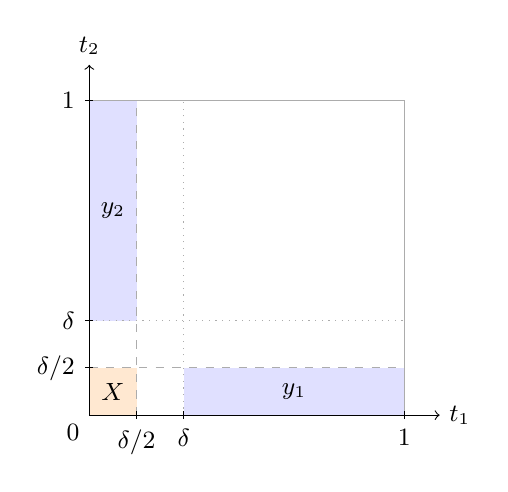
\begin{tikzpicture}[x=1cm,y=1cm,font=\small]
  \fill[orange!18] (0,0) rectangle (0.6,0.6);
  \fill[blue!12] (1.2,0) rectangle (4,0.6);
  \fill[blue!12] (0,1.2) rectangle (0.6,4);
  \draw[gray!65,thin] (0,0) rectangle (4,4);
  \draw[gray!65,dashed,thin] (0.6,0) -- (0.6,4);
  \draw[gray!65,dashed,thin] (0,0.6) -- (4,0.6);
  \draw[gray!65,dotted,thin] (1.2,0) -- (1.2,4);
  \draw[gray!65,dotted,thin] (0,1.2) -- (4,1.2);
  \draw[->] (0,0) -- (4.45,0) node[right] {$t_1$};
  \draw[->] (0,0) -- (0,4.45) node[above] {$t_2$};
  \node[below left] at (0,0) {$0$};
  \foreach \x/\ticktext in {0.6/{\delta/2},1.2/{\delta},4/{1}} {
    \draw (\x,0.05) -- (\x,-0.05);
    \node[below] at (\x,-0.06) {$\ticktext$};
    \draw (0.05,\x) -- (-0.05,\x);
    \node[left] at (-0.06,\x) {$\ticktext$};
  }
  \node at (0.3,0.3) {$X$};
  \node at (2.6,0.3) {$y_1$};
  \node at (0.3,2.6) {$y_2$};
\end{tikzpicture}

\caption{Support geometry for \(k=2\), drawn schematically. Shading
shows the closures of the regions where \(X\), \(y_1\), and \(y_2\)
can be nonzero. In the \(y_j\) region, \(r(t)\) is the \(j\)-th vertex
and \(H(t)=1\), giving \eqref{eq:cone-local-support}.}
\label{fig:cone-support}
\end{figure}

Use the same letters for the images of these elements under
\(\eta^{\otimes k}:C^{\otimes k}\to P^{\otimes k}\), and put
\(Y=\sum_{j=1}^k y_j\). All the identities just proved persist.
Writing \(G=\eta(g)\), we have
\([G]\le[1_P]\le N[c]\).
Tensor this comparison with \(G\) in the other \(k-1\) positions to
obtain
\[
[X]\le N[y_j]\quad(1\le j\le k).
\]
Adding these comparisons and using orthogonality gives
\begin{equation}\label{eq:cone-defect-sum}
k[X]\le N\sum_{j=1}^k[y_j]=N[Y].
\end{equation}
Thus the cube supplies \(k\) copies of the defect below \(N\) copies of
an element supported where \(a_1=1\). The auxiliary algebra \(R\) was
chosen precisely to remove these unequal multiplicities without any
cancellation in the Cuntz order.

\emph{Absorbing the defect.}
Finally, work in
\[
B=P^{\otimes k}\otimes R=P^{\otimes(k+L)},
\qquad b_i=a_i\otimes1_R.
\]
Since \(a_1Y=Y\), taking adjoints gives \(Ya_1=Y\).
Thus \(a_1\) and \(Y\) commute, and functional calculus gives
\((a_1-1/2)_+Y=Y/2\). In particular the element
\(z=\sqrt{2Y}\otimes1_R\) satisfies
\[
z^*(b_1-1/2)_+z=Y\otimes1_R.
\]
The following use of tensor divisibility to obtain comparison follows
the pattern of Robert and R\o rdam \cite[Lemma~6.1(i)]{RR}; we verify the
comparisons directly in maximal tensor products. Together with
\eqref{eq:cone-amplification} and
\eqref{eq:cone-defect-sum}, this yields
\[
\begin{aligned}
[X\otimes1_R]
&\le k[X\otimes e]\\
&\le N[Y\otimes e]\\
&\le[Y\otimes1_R]\\
&\le[(b_1-1/2)_+].
\end{aligned}
\]
The first comparison tensors \([1_R]\le k[e]\) with \(X\), the
second tensors \eqref{eq:cone-defect-sum} with \(e\), and the third
tensors \(N[e]\le[1_R]\) with \(Y\). The last uses the exact witness
\(z\). These are comparisons in finite matrices over the maximal
tensor product \(B\).

To express the conclusion inside \(B\) itself, recall that if
\(a,b\in B_+\) and
\[
W_n^*(b\oplus0)W_n\longrightarrow a\oplus0
\]
in finite matrices, compression to the upper-left corner gives
\((W_n)_{11}^*b(W_n)_{11}\to a\).
The final comparison therefore gives
\[
1_B-b_1-b_2=X\otimes1_R\precsim(b_1-1/2)_+
\quad\text{in }B.
\]
By \eqref{eq:cone-positive-pair}, the elements \(b_1,b_2\) are
orthogonal positive contractions with exact equivalence witness
\(v_B=v\otimes1_R\in B\). This proves the asserted pair and defect
comparison. Proposition~\ref{prop:rw}, with cutoff \(1/2\),
now gives a unital \(*\)-homomorphism \(I(2,3)\to B\).
Taking \(m=k+L\) completes the proof.
\end{proof}

\section{From finite tensor powers to absorption}\label{sec:application}

\begin{proof}[Proof of Theorem~\ref{thm:finite}]
Proposition~\ref{prop:full-cone} supplies a finite tensor power
$P=D^{\otimes m_0}$ and a unital map $\eta:C\to P$ for which
$\eta(\iota e_{11})$ is full. Proposition~\ref{prop:cone-drop} supplies a
unital map from $I(2,3)$ into a finite tensor power $P^{\otimes s}$.
Associativity of the maximal tensor product identifies the latter with
$D^{\otimes m_0s}$, as required.
\end{proof}

For the application, we first record explicitly why the possibly
nonseparable central-sequence algebra contains a suitable separable
subalgebra. This is the separable-reduction argument of
\cite[Lemma~3.5]{KR}; we include its finite commutator witness.

\begin{lemma}\label{lem:separable}
Every nonzero unital $C^*$-algebra $B$ without characters contains a
separable $C^*$-subalgebra $D$ without characters and with $1_D=1_B$.
\end{lemma}
\begin{proof}
The closed ideal generated by commutators of selfadjoint elements is $B$;
a proper such ideal would give a nonzero unital commutative quotient and
hence a character. Consequently, there are finitely many
$h_i,k_i\in B$ and $b_i,c_i\in B_{\sa}$ such that
\[
 \left\|1_B-\sum_{i=1}^r h_i[b_i,c_i]k_i\right\|<1.
\]
Let $D$ be generated by $1_B$ and all the displayed elements. It is unital
and separable. A character of $D$ would send the sum to zero and the unit
to one, contradicting its contractivity and the strict norm bound.
\end{proof}

\begin{proof}[Proof of Theorem~\ref{thm:main}]
Assume that $F_\omega(A)$ has no characters. This algebra is nonzero and
unital because it contains the diagonal unit of $A$. By
Lemma~\ref{lem:separable}, choose a separable unital characterless
subalgebra $D\subset F_\omega(A)$ with the same unit. By
Theorem~\ref{thm:finite} and Proposition~\ref{prop:kr}(1), there is a
composition of unital $*$-homomorphisms
\[
 I(2,3)\longrightarrow D^{\otimes_{\max}m}
 \longrightarrow F_\omega(A).
\]
Denote its image by $E$. The image is separable and is a quotient of
$I(2,3)$. Every irreducible representation of $I(2,3)$ factors through
evaluation at a point of $[0,1]$: the central algebra $C([0,1])1$ acts
by a character, and sections vanishing at its evaluation point are
annihilated, by approximation using scalar functions vanishing there.
The resulting irreducible dimensions are $2$ at $0$, $3$ at $1$, and
$6$ in the interior. Thus $I(2,3)$ is subhomogeneous and has no
characters. The same properties hold for $E$, since any irreducible
representation or character of $E$ pulls back along the quotient map.
Also $1_E=1_{F_\omega(A)}$. Proposition~\ref{prop:kr}(2) gives
$A\cong A\otmin\Z$.

Conversely, if $A\cong A\otmin\Z$, Proposition~\ref{prop:kr}(2)
supplies a unital subalgebra $E\subset F_\omega(A)$ without characters.
Any character of $F_\omega(A)$ would restrict to a character of $E$,
a contradiction.
\end{proof}

\begin{proof}[Proof of Corollary~\ref{cor:infinite-tensor}]
Because $D$ is nonzero and unital, each spatial connecting map
$x\mapsto x\otimes1_D$ is a unital embedding. Thus $B$ is nonzero, unital,
and separable, and the canonical maps
$\iota_m:D^{\otimes_{\min}m}\hookrightarrow B$ are unital.
Choose the unital homomorphism $\phi$ from Theorem~\ref{thm:finite} and
compose it with the canonical maximal-to-minimal quotient and the
finite-stage inclusion:
\[
 I(2,3)\xrightarrow{\ \phi\ }D^{\otimes_{\max}m}
 \xrightarrow{\ q_m\ }D^{\otimes_{\min}m}
 \xrightarrow{\ \iota_m\ }B.
\]
The quotient $q_m$ is unital, with no nuclearity assumption on $D$.
Let $\theta$ denote this composite and put $E=\theta(I(2,3))$.
Since $\theta$ is unital, $1_E=1_B\ne0$.
The algebra $I(2,3)$ is separable and, as checked above, subhomogeneous
and characterless. Its quotient $E\cong I(2,3)/\ker\theta$ is therefore
separable and subhomogeneous: every irreducible representation of $E$
pulls back to one of $I(2,3)$. A character of $E$ would compose with the
unital quotient map to a character of $I(2,3)$, which is impossible.
These conclusions hold even when $\theta$ has a kernel.

Dadarlat--Toms \cite[Theorem~1.1]{DT}, applied to the unital separable
algebra $D$ and this same-unit subalgebra of $B$, gives
$B\cong B\otmin\Z$. Finally, because $B\ne0$, the map
$z\mapsto1_B\otimes z$ embeds $\Z$ unitally into $B\otmin\Z$.
Transporting this map through the inverse of an isomorphism
$B\cong B\otmin\Z$, which is automatically unital, gives the asserted
unital copy of $\Z$ in $B$.
\end{proof}

\begin{thebibliography}{STW}
\raggedright

\bibitem[DT]{DT}
Marius Dadarlat and Andrew S. Toms,
\emph{$\mathcal Z$-stability and infinite tensor powers of $C^*$-algebras},
Adv. Math. \textbf{220} (2009), 341--366.
\href{https://doi.org/10.1016/j.aim.2008.07.002}{doi:10.1016/j.aim.2008.07.002}.

\bibitem[JS]{JS}
Xinhui Jiang and Hongbing Su,
\emph{On a simple unital projectionless $C^*$-algebra},
Amer. J. Math. \textbf{121} (1999), no.~2, 359--413.
\href{https://doi.org/10.1353/ajm.1999.0012}{doi:10.1353/ajm.1999.0012}.

\bibitem[KR]{KR}
Eberhard Kirchberg and Mikael R\o rdam,
\emph{When central sequence $C^*$-algebras have characters},
Internat. J. Math. \textbf{26} (2015), no.~7, 1550049, 32~pp.
\href{https://doi.org/10.1142/S0129167X15500494}{doi:10.1142/S0129167X15500494}.
\href{https://arxiv.org/abs/1409.1395v2}{arXiv:1409.1395v2}.

\bibitem[OAI]{Fixed231}
OpenAI,
\emph{Nuclear dimension and Jiang--Su stability without elementary
subquotients},
OpenAI Math Release preprint
\href{https://github.com/openai/math/blob/main/preprints/Nuclear-dimension-and-Jiang-Su-stability-without-elementary-subquotients-September-23-2026/paper.pdf}{OAI:Nuclear-dimension-and-Jiang-Su-stability-without-elementary-subquotients-September-23-2026},
2026.
Theorem~1.4 and Lemma~9.3.

\bibitem[PTV]{PTV}
Francesc Perera, Hannes Thiel, and Eduard Vilalta,
\emph{Centrally pure $C^*$-algebras},
preprint, submitted December~19, 2025.
\href{https://arxiv.org/abs/2512.17261v1}{arXiv:2512.17261v1}.
Online journal publication:
\href{https://doi.org/10.1016/j.jfa.2026.111578}{doi:10.1016/j.jfa.2026.111578}.

\bibitem[RR]{RR}
Leonel Robert and Mikael R\o rdam,
\emph{Divisibility properties for $C^*$-algebras},
Proc. Lond. Math. Soc. (3) \textbf{106} (2013), no.~6, 1330--1370.
\href{https://doi.org/10.1112/plms/pds082}{doi:10.1112/plms/pds082}.

\bibitem[RT]{RT}
Leonel Robert and Aaron Tikuisis,
\emph{Nuclear dimension and $\mathcal Z$-stability of non-simple
$C^*$-algebras},
Trans. Amer. Math. Soc. \textbf{369} (2017), no.~7, 4631--4670.
\href{https://doi.org/10.1090/tran/6842}{doi:10.1090/tran/6842}.

\bibitem[RW]{RW}
Mikael R\o rdam and Wilhelm Winter,
\emph{The Jiang--Su algebra revisited},
J. Reine Angew. Math. \textbf{642} (2010), 129--155.
\href{https://doi.org/10.1515/crelle.2010.039}{doi:10.1515/crelle.2010.039}.
\href{https://web.math.ku.dk/~rordam/manus/jiang-su-revisited.pdf}{Author manuscript},
January~27, 2009.

\bibitem[STW]{STW}
Christopher Schafhauser, Aaron Tikuisis, and Stuart White,
\emph{Nuclear $C^*$-algebras: 99 problems},
preprint, 2025, revised May~8, 2026.
\href{https://arxiv.org/abs/2506.10902v2}{arXiv:2506.10902v2}.

\bibitem[TW]{TW}
Andrew S. Toms and Wilhelm Winter,
\emph{Strongly self-absorbing $C^*$-algebras},
Trans. Amer. Math. Soc. \textbf{359} (2007), no.~8, 3999--4029.
\href{https://doi.org/10.1090/S0002-9947-07-04173-6}{doi:10.1090/S0002-9947-07-04173-6}.

\bibitem[WZ]{WZ}
Wilhelm Winter and Joachim Zacharias,
\emph{Completely positive maps of order zero},
M\"unster J. Math. \textbf{2} (2009), 311--324.
\href{https://www.uni-muenster.de/FB10/mjm/vol_2/mjm_vol_2_14.pdf}{Published version}.

\end{thebibliography}

\end{document}
